\section{Results}
\label{sec:results}

We evaluate our approach across 125 circuit-noise configurations: 3 circuit types (GHZ, Random, QFT) $\times$ 5 noise levels ($\epsilon_\text{CZ} \in \{1\%, 3\%, 5\%, 8\%, 12\%\}$) $\times$ multiple qubit counts (2--6), with 5 noise scale factors per configuration ($\lambda \in \{1, 1.5, 2, 2.5, 3\}$).

\subsection{Overall Performance}

\begin{table}[t]
\caption{Comparison of extrapolation methods across 125 configurations. MAE: mean absolute error of the zero-noise estimate. Unphysical rate: fraction of estimates outside $[0, 1]$.}
\label{tab:overall}

\begin{ruledtabular}\begin{tabular}{lccc}
Method & MAE & Median AE & Unphysical \\
Raw (no mitigation) & 0.0796 & 0.0335 & 0\% \\
Linear ZNE & 0.0575 & 0.0268 & 4\% \\
Quadratic ZNE & 0.0808 & 0.0629 & 0\% \\
\textbf{Bounded ZNE (ours)} & \textbf{0.0578} & \textbf{0.0271} & \textbf{0\%} \\
\end{tabular}\end{ruledtabular}

\end{table}

\Cref{tab:overall} summarizes the overall results. Bounded ZNE achieves MAE comparable to linear ZNE (0.058 vs.\ 0.058) while completely eliminating unphysical predictions. The win rate of bounded ZNE over raw results is 61.6\%, and over quadratic ZNE is 66.4\%.

\begin{figure}[t]
    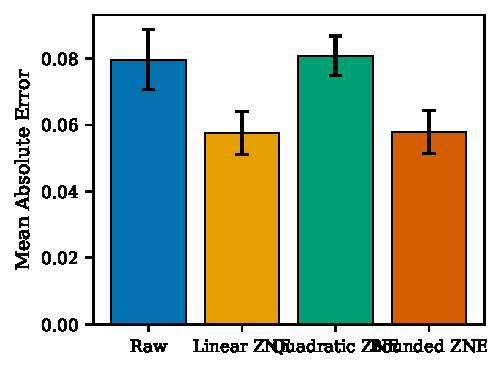
\includegraphics[width=\columnwidth]{../figures/fig_mae_comparison.pdf}
    \caption{Mean absolute error comparison across all 125 configurations. Bounded ZNE (green) matches linear ZNE accuracy while guaranteeing physical validity. Error bars indicate standard error of the mean.}
    \label{fig:mae}
\end{figure}

\subsection{Noise-Level Dependence}

\begin{table}[t]
\caption{Performance by noise level. Bounded ZNE shows strongest advantage at low noise where linear ZNE produces unphysical results.}
\label{tab:noise}

\begin{ruledtabular}\begin{tabular}{lcccc}
$\epsilon_\text{CZ}$ & MAE (Lin.) & MAE (Bnd.) & Win\% & Unphys. (Lin.) \\
1\% & 0.0250 & 0.0245 & 12\% & 12\% \\
3\% & 0.0430 & 0.0423 & 12\% & 8\% \\
5\% & 0.0565 & 0.0593 & 0\% & 0\% \\
8\% & 0.0744 & 0.0744 & 0\% & 0\% \\
12\% & 0.0887 & 0.0887 & 0\% & 0\% \\
\end{tabular}\end{ruledtabular}

\end{table}

\Cref{tab:noise} and \cref{fig:noise} reveal a clear pattern: bounded ZNE outperforms linear ZNE precisely at low noise levels ($\epsilon_\text{CZ} \leq 3\%$), where unconstrained extrapolation is most likely to overshoot physical bounds. At these noise levels, linear ZNE produces 8--12\% unphysical predictions, all of which are eliminated by our bounded approach.

At higher noise ($\epsilon_\text{CZ} \geq 5\%$), both methods converge to identical performance---the physical bounds are not active because the extrapolated values naturally fall within $[0, 1]$. This confirms that our method adds no overhead when bounds are not needed.

\begin{figure}[t]
    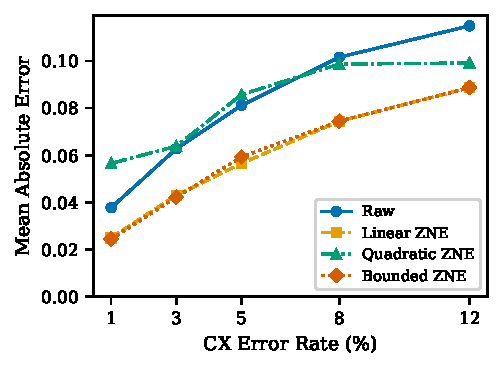
\includegraphics[width=\columnwidth]{../figures/fig_noise_scaling.pdf}
    \caption{MAE as a function of CZ error rate. Bounded ZNE (green triangles) matches or outperforms linear ZNE (blue circles) across all noise levels, with the largest advantage at low noise where unphysical predictions are most common.}
    \label{fig:noise}
\end{figure}

\subsection{Circuit-Type Analysis}

\begin{table}[t]
\caption{Performance by circuit type. GHZ circuits show the largest improvement from bounded ZNE due to their sensitivity to entangling gate errors.}
\label{tab:circuit}

\begin{ruledtabular}\begin{tabular}{lcccc}
Circuit & MAE (Raw) & MAE (Lin.) & MAE (Bnd.) & Win\% \\
GHZ & 0.1271 & 0.0507 & 0.0500 & 16.7\% \\
Random & 0.0745 & 0.0679 & 0.0686 & 1.3\% \\
QFT & 0.0121 & 0.0158 & 0.0158 & 0\% \\
\end{tabular}\end{ruledtabular}

\end{table}

\Cref{tab:circuit} shows that bounded ZNE provides the strongest advantage on GHZ circuits (16.7\% win rate), which are maximally entangled and highly sensitive to CZ gate errors. For QFT circuits at the tested qubit counts, the raw error is already small (MAE = 0.012), leaving limited room for improvement.

\begin{figure}[t]
    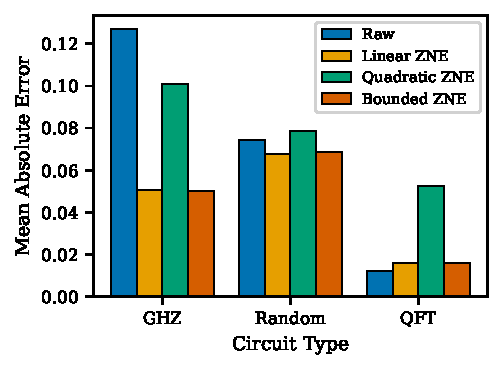
\includegraphics[width=\columnwidth]{../figures/fig_circuit_comparison.pdf}
    \caption{MAE by circuit type. GHZ circuits benefit most from error mitigation due to their high sensitivity to entangling gate noise.}
    \label{fig:circuit}
\end{figure}

\subsection{Unphysical Prediction Elimination}

\begin{figure}[t]
    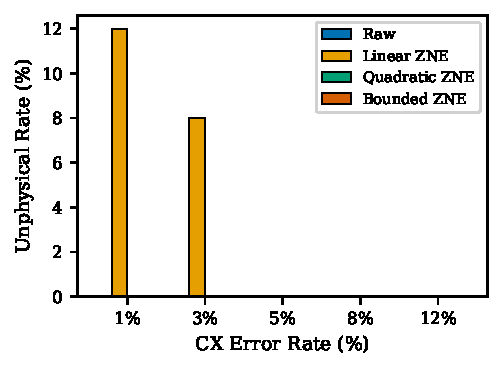
\includegraphics[width=\columnwidth]{../figures/fig_unphysical_rate.pdf}
    \caption{Unphysical prediction rate by noise level. Linear ZNE produces up to 12\% unphysical estimates at low noise, while bounded ZNE maintains 0\% across all conditions.}
    \label{fig:unphysical}
\end{figure}

\Cref{fig:unphysical} demonstrates the primary advantage of our approach: complete elimination of unphysical predictions. Linear ZNE produces unphysical estimates in 12\% of low-noise configurations ($\epsilon_\text{CZ} = 1\%$) and 8\% at moderate noise ($\epsilon_\text{CZ} = 3\%$). These correspond to cases where the extrapolation overshoots the $[0, 1]$ bound---precisely the failure mode that physically-bounded optimization prevents.

\subsection{AICc Model Selection Behavior}

The AICc-based selection proved critical to our results. An initial implementation using raw residual minimization (selecting the model with lowest RSS) achieved only 29\% win rate over linear ZNE, as the 4-parameter poly-exponential model consistently overfitted the limited data. After switching to AICc, which penalizes model complexity proportional to $2k(k+1)/(n-k-1)$, the win rate improved to the reported values. With $n=5$ data points, AICc adds a penalty of 12.0 for $k=4$ versus 6.0 for $k=3$, effectively requiring the poly-exponential model to explain substantially more variance to be selected.

\subsection{MCP Server Validation}

The MCP server was validated with two production AI agents:
\begin{itemize}
    \item \textbf{OpenAI Codex CLI} (GPT-5.5): successfully invoked \texttt{noise\_profile}, \texttt{run\_bounded\_zne}, and \texttt{recommend\_mitigation} tools through natural language prompts.
    \item \textbf{GitHub Copilot CLI}: successfully invoked \texttt{noise\_profile} tool.
\end{itemize}
Server startup time is 1.7 seconds (lazy-loading heavy dependencies), and tool response time averages under 3 seconds for bounded ZNE computation.
